\begin{figure}[H]
  \centering
  \label{tikzpic:composite_functions}
  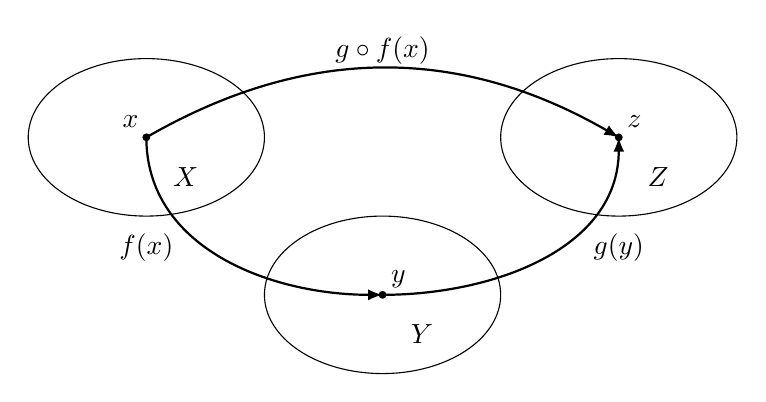
\begin{tikzpicture}[>= latex]
    \draw (-3 cm, 0) ellipse (1.5 cm and 1 cm);
    \draw ( 3 cm, 0) ellipse (1.5 cm and 1 cm);
    \draw ( 0   , -2 cm) ellipse (1.5 cm and 1 cm);

    \draw (-3, -1.4) node {$f(x)$};
    \draw[thick, ->] (-3, 0) to [out = -90, in = 180] (0, -2);

    \draw (3, -1.4) node {$g(y)$};
    \draw[thick, ->] (0, -2) to [out = 0, in = -90] (3, 0);

    \draw (0, 1.1) node {$g \circ f(x)$};
    \draw[thick, ->] (-3, 0) to [out = 30, in = 150] (3, 0);

    \fill (-3,0) circle (0.05);
    \draw (-3.2,.2) node {$x$};
    \draw (-2.5,-.5) node {$X$};

    \fill (0,-2) circle (0.05);
    \draw (0.2,-1.8) node {$y$};
    \draw (0.5,-2.5) node {$Y$};

    \fill (3,0) circle (.05);
    \draw (3.2,.2) node {$z$};
    \draw (3.5,-.5) node {$Z$};
  \end{tikzpicture}
  \caption{Композиция функций}
\end{figure}

